\documentclass[conference]{IEEEtran}
\IEEEoverridecommandlockouts
% The preceding line is only needed to identify funding in the first footnote. If that is unneeded, please comment it out.
\usepackage{cite}
\usepackage{amsmath,amssymb,amsfonts}
\usepackage{algorithmic}
\usepackage{graphicx}
\usepackage{textcomp}
\usepackage{xcolor}
\def\BibTeX{{\rm B\kern-.05em{\sc i\kern-.025em b}\kern-.08em
    T\kern-.1667em\lower.7ex\hbox{E}\kern-.125emX}}
\begin{document}

\title{Paxos: An Evaluation
}

\author{\IEEEauthorblockN{Aakash Sharma}
\IEEEauthorblockA{\textit{Department of Computer Science \\
\textit{UiT -- The Arctic University of Norway}\\
Troms{\o}, Norway \\
aakash.sharma@uit.no}
}
}

\maketitle

\begin{abstract}
This report provides an evaluation study of Paxos algorithm from a systems perspective. 
The evaluation is based on an implementation of Paxos~\cite{b3} in python.
Various parameters were modified to understand different behaviors of reaching consensus using Paxos algorithm. 
Various evaluation parameters are presented and the results are discussed in this report. 
The evaluation was performed using a single machine running the \textit{replica} nodes and the \textit{leader} nodes. 
\end{abstract}

\begin{IEEEkeywords}
Distributed System, Consensus, Fault Tolerance
\end{IEEEkeywords}

\section{Introduction}
Paxos was proposed by Leslie Lamport in his paper "Part-time Parliament" \cite{b1}. 
The algorithm provides a way to reach consensus in a system with multiple participating nodes. 
The working principle behind Paxos algorithm is that the proposer node receives a \textit{propose}, it sends a prepare message to all of the \textit{acceptor} nodes which contains the Paxos iteration number and the proposal number. 
The acceptor node on receiving such message can reply with a rejection or with a \textit{promise}. 
A \textit{promise} is a guarantee that the \textit{acceptor} node will not accept another proposal from any proposer node with a lower proposal number. 
If the proposer receives promise messages from a majority of the acceptor nodes, it can move forward with the actual proposal message. 
The proposer node then sends a message containing Paxos iteration number, the proposal number and the proposal value to the acceptors. 
If the proposer node receives Accept from majority of acceptor nodes, the iteration will end resulting in the network reaching a consensus on the value. 
\section{Experiments and Results}
%\begin{figure}
%	\label{fig:paxos}
%	\centering
%	\vspace*{-3cm}
%	\includegraphics[scale=.45]{output} 
%	\vspace*{-3.5cm}
%	\caption{Scalability of Paxos Algorithm}
%\end{figure}
For the evaluation, we used the Paxos implementation by van Renesse \& Altinbuken \cite{b3}. 
The evaluation is designed to determine the scalability of the Paxos algorithm by increasing the amount of participating nodes in the consensus. 
The throughput is measured as the number of consensus reached per second. 
For the evaluation, multiple sets of the test runs are evaluated in order to achieve average performance indicators. 
For this study, we have used 4 test runs. 
The system used for evaluation is powered by an Intel 7700HQ processor clocked at a frequency of 2.8 GHz. 
The system has 16 GB of RAM and running MacOS version 10.14.3. 
The implementation is running on Python 2.7.10 interpreter. \\

\begin{figure}[!h]
	\label{figure1}
	\centering
	\vspace*{-3cm}
	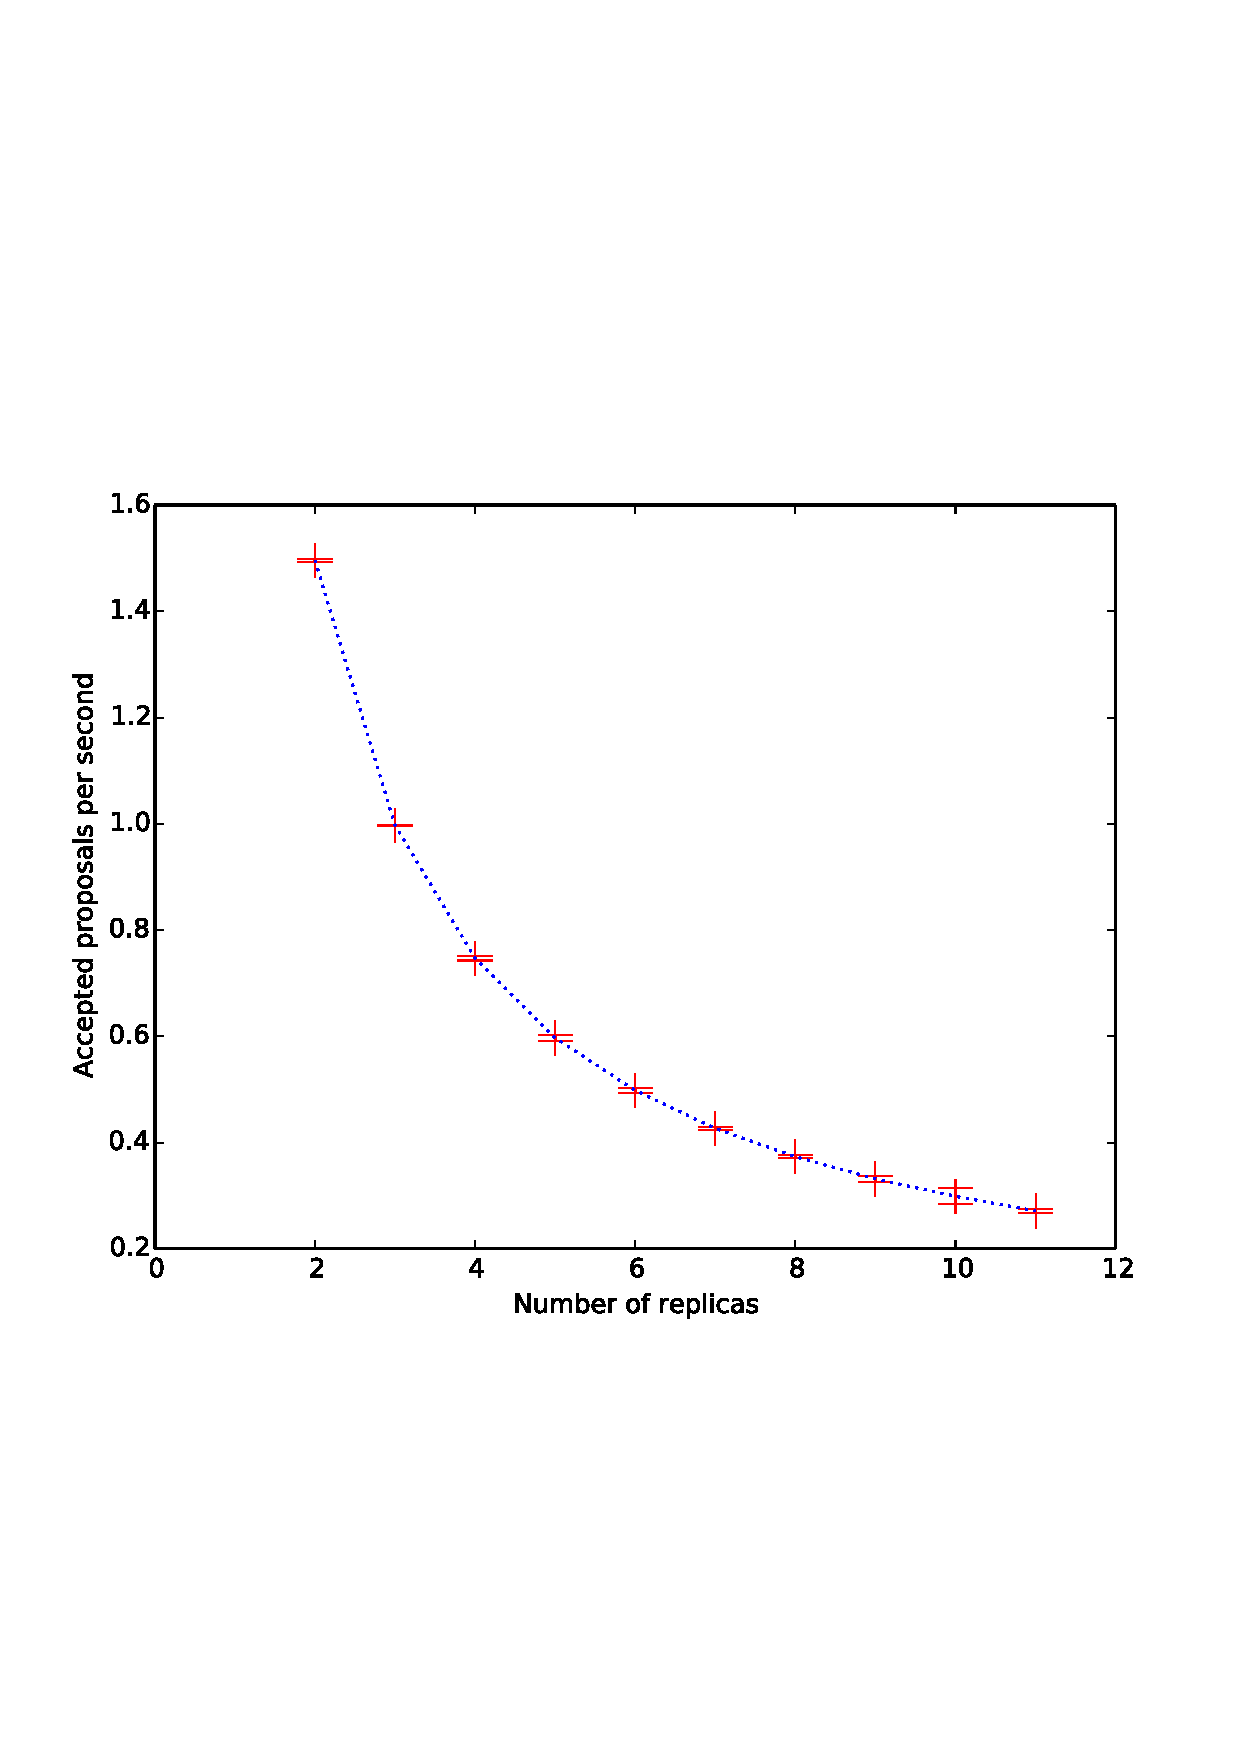
\includegraphics[scale=.45]{figure1}
	\vspace*{-3cm}
	\caption{Accepted proposals per second vs. the number of replicas in the Paxos cluster}
\end{figure}

The results of the evaluation are plotted in Figure \ref{figure1}. 
As expected, with the increasing number of consensus nodes in the network, the throughput of the system declines. 
This is inline with the expectation that the proposer node has to wait for sufficient promise messages to form a majority in the system. 
Similarly, before committing the proposer again waits for enough Accept messages from the participating nodes to obtain a majority. 
The amount of messages induces increased time to reach consensus and thereby reducing the overall throughput of the system. 
Work by Santos and Schiper \cite{b2} has suggested batching and pipelining to increase the overall throughput of a Paxos based system. 
\section{Conclusion}
In this work, we have studied the scalability of the Paxos algorithm. The result shows reduced throughput with an increasing number of participating nodes. 


\section*{References}
%\bibliographystyle{ieee}
%\bibliography{bibli}

\begin{thebibliography}{00}
\bibitem{b1} Lamport, Leslie. "The part-time parliament." ACM Transactions on Computer systems 16.2 (1998): 133-169.
\bibitem{b2} Santos, Nuno, and André Schiper. "Tuning paxos for high-throughput with batching and pipelining." International Conference on Distributed Computing and Networking. Springer, Berlin, Heidelberg, 2012.
\bibitem{b3}Van Renesse, Robbert, and Deniz Altinbuken. "Paxos Made Moderately Complex." ACM Comput. Surv. 47.3 (2015): 42-1.
\end{thebibliography}
%\vspace{12pt}
%\color{red}
%IEEE conference templates contain guidance text for composing and formatting conference papers. Please ensure that all template text is removed from your conference paper prior to submission to the conference. Failure to remove the template text from your paper may result in your paper not being published.

\end{document}
